% SPDX-License-Identifier: MIT
% Original A4 two-column research-paper source.
\documentclass[10pt,a4paper,twocolumn]{article}
\usepackage[margin=18mm,top=17mm,bottom=19mm,columnsep=7mm]{geometry}
\usepackage{fontspec}
\setmainfont{Arial}
\setmonofont{Consolas}
\usepackage{microtype,booktabs,tabularx,array,amsmath,enumitem,xcolor,url}
\usepackage{tikz}
\usetikzlibrary{arrows.meta,positioning,fit}
\usepackage[colorlinks=true,linkcolor=black,urlcolor=blue!55!black,citecolor=blue!55!black]{hyperref}
\usepackage[nameinlink,noabbrev]{cleveref}
\usepackage{fancyhdr,lastpage}
\setlength{\parindent}{0pt}\setlength{\parskip}{.25em}
\setlist{nosep,leftmargin=1.2em}
\renewcommand{\familydefault}{\sfdefault}
\definecolor{accent}{HTML}{1E4E79}\definecolor{light}{HTML}{F3F6F8}
\pagestyle{fancy}\fancyhf{}
\lhead{\footnotesize Distributed Fraud Detection Engine}
\rhead{\footnotesize Research note}
\cfoot{\footnotesize \thepage\ / \pageref{LastPage}}
\renewcommand{\headrulewidth}{.25pt}
\newcommand{\code}[1]{\texttt{#1}}
\newcommand{\nm}{\textbf{not measured}}
\newcolumntype{Y}{>{\raggedright\arraybackslash}X}
\hypersetup{pdftitle={Evidence-First Design of a Distributed Fraud Detection Engine},pdfauthor={Distributed Fraud Detection project}}

\begin{document}
\twocolumn[
\begin{center}
{\LARGE\bfseries Evidence-First Design of a Distributed Fraud Detection Engine\par}
\vspace{3pt}
{\large Shared-Memory ABI, Deadline-Aware Batching, and GPU Execution Methodology\par}
\vspace{9pt}
{\normalsize Project research note\par}
{\small Implementation-aligned design document \quad | \quad 30 July 2026\par}
\vspace{9pt}\rule{.92\textwidth}{.35pt}
\end{center}\vspace{5pt}
]
\begin{abstract}
Fraud scoring on an authorization path is judged by tail latency, bounded failure
behavior, and auditability as much as model accuracy. This paper documents an
implementation-aligned design: a Rust gateway serializes a fixed request into a
System V shared-memory slot; a native daemon consumes it through a bounded MPMC
ring; and a deadline-aware batcher dispatches compact batches to a capability-
gated GPU path. The design separates the synchronous path from streaming
aggregation, training, and rollout. It specifies a stable ABI, allocation
boundaries, sequence-number ownership, and a reproducible protocol based on
open-loop Poisson arrivals and HDR histograms. Two bounded evidence sets are
reported. Five local RTX 3050 component runs found no benefit for the tiny
launch-dominated graph stub: direct and graph-replay p99 were 58.1 and
59.5~$\mu$s. One seeded Linux CPU-reference run completed 15,000 authenticated
HTTP/shared-memory decisions at 1,500 requests/s with no errors, p50 2.325~ms,
p99 3.421~ms, and p99.9 3.939~ms. These are not full-model production results;
V0=150~ms through V3=4~ms remain historical/design targets.
\end{abstract}

\section{Problem and service-level boundary}
An authorization decision must arrive before its caller's deadline, with clear
provenance for both primary and degraded outcomes. The engine returns an allow,
review, or decline recommendation from a bounded transaction representation. Its
low-latency objective applies only to a warm, co-located scoring path inside one
region. Ingestion, feature backfill, training, promotion, cold start, and
cross-region calls are outside that boundary. Tail latency is whole-path
behavior: a fast kernel cannot compensate for queueing, cache misses, or a
network hop.

The target inherits the tail-at-scale problem: fan-out makes an infrequent slow
component visible to a user-facing tail \cite{dean2013}. Each request has one
absolute deadline. Gateway validation, one fixed-width feature read, scheduler
queueing, worker dispatch, and encoding consume shrinking child budgets; work is
not begun after expiration. A timeout or unhealthy worker returns a deterministic,
auditable fallback when a trustworthy feature block exists, and fails closed
when it does not.

\begin{table}[t]\centering\small
\caption{Latency scope and current evidence status.}\label{tab:scopes}
\begin{tabularx}{\columnwidth}{@{}lY@{}}\toprule
Scope & Definition and status \\\midrule
Kernel & Nsight GPU activity for the warmed forward stub: median 0.864~$\mu$s
($n=2{,}100$); not a full model. \\
Batch call & CPU wall time around warmed batch-32 copy/forward/synchronize:
direct p99 58.1~$\mu$s; graph p99 59.5~$\mu$s. \\
API decision & Planned client arrival through HTTP response on one CPU-only
GitHub runner: p99 3.421~ms ($n=15{,}000$). \\\bottomrule
\end{tabularx}\end{table}

\subsection{Historical versions are not results}
The project brief's V0--V5 sequence is a decision plan. V0 (naive PyTorch API),
V1 (C++ API over TCP), V2 (shared-memory IPC), and V3 (CUDA Graphs plus pinned
memory) identify intended comparisons; V4 and V5 need frozen definitions before
measurement. The values V0=150 ms, V1=45 ms, V2=12 ms, and V3=4 ms are
historical/design targets only. No like-for-like manifest proves them, so they
are neither observed latency nor an SLA. The repository's 1 ms warm/co-located
phase budget is also prospective.

\begin{table}[t]\centering\small
\caption{Historical target ledger, not measured results.}\label{tab:targets}
\begin{tabularx}{\columnwidth}{@{}clYp{.27\columnwidth}@{}}\toprule
Version & Value & Stage & Interpretation \\\midrule
V0 & 150 ms & naive PyTorch API & historical target \\
V1 & 45 ms & C++ API / TCP & historical target \\
V2 & 12 ms & shared-memory IPC & historical target \\
V3 & 4 ms & graph / pinned memory & historical target \\
V4 & -- & calibrated low precision & definition needed \\
V5 & -- & fused short context & definition needed \\\bottomrule
\end{tabularx}\end{table}

\section{Architecture}
The warm path authenticates and bounds the payload, materializes one fixed-width
feature vector, reserves a daemon slot, and waits only until the inherited
deadline. The daemon batches ready slots and executes a CPU reference handler or
a separately enabled CUDA/CUTLASS integration. The stream processor is off the
critical path: it maintains event-time state and writes materialized features
for later reads.

\begin{figure*}[t]\centering
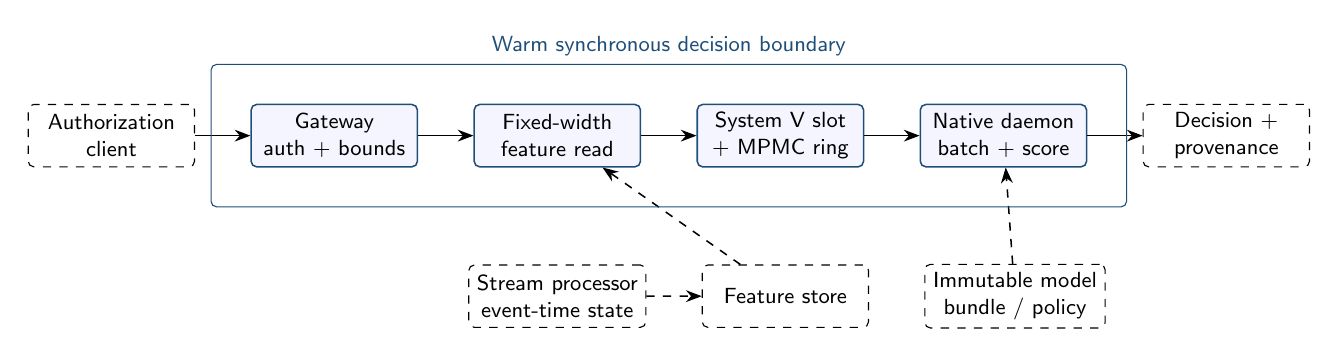
\begin{tikzpicture}[font=\small,node distance=7mm and 8mm,scale=.88,transform shape,
box/.style={draw,rounded corners=2pt,minimum height=9mm,minimum width=24mm,align=center,fill=light},
hot/.style={box,draw=accent,line width=.55pt,fill=blue!4},ext/.style={box,dashed,fill=white},
arrow/.style={-{Stealth[length=2mm]},line width=.55pt}]
\node[ext](c){Authorization\\client};
\node[hot,right=of c](g){Gateway\\auth + bounds};
\node[hot,right=of g](f){Fixed-width\\feature read};
\node[hot,right=of f](r){System V slot\\+ MPMC ring};
\node[hot,right=of r](d){Native daemon\\batch + score};
\node[ext,right=of d](o){Decision +\\provenance};
\draw[arrow](c)--(g);\draw[arrow](g)--(f);\draw[arrow](f)--(r);\draw[arrow](r)--(d);\draw[arrow](d)--(o);
\node[ext,below=14mm of f](s){Stream processor\\event-time state};
\node[ext,right=of s](store){Feature store};
\node[ext,right=of store](m){Immutable model\\bundle / policy};
\draw[arrow,dashed](s)--(store);\draw[arrow,dashed](store)--(f);\draw[arrow,dashed](m)--(d);
\node[draw=accent,rounded corners=2pt,fit=(g)(d),inner sep=5mm,label={[accent]above:Warm synchronous decision boundary}]{};
\end{tikzpicture}
\caption{Architecture and latency boundary. Dashed elements affect correctness or availability but are not sequential warm-request stages.}\label{fig:architecture}
\end{figure*}

The deployment model uses ready replicas, health/circuit routing, immutable model
artifacts, TLS-protected dependencies, and explicit fallback labels. It does not
promise exactly-once multi-writer aggregation; Kafka transactions, durable state,
and Redis version fencing remain prerequisites. Nor does it claim the local CPU
scorer is an exported production transformer.
\section{ABI and zero-copy handoff}
The interprocess contract is a versioned binary ABI, not a C++ object layout.
The daemon creates a mode-0600 System V segment; the gateway locates it with
\code{shmget} and attaches with \code{shmat}. Their lifecycle and permission
semantics are documented by Linux \cite{linuxshmget,linuxshmat}. The header begins
with magic \code{0x46444950} (FDIP), version 1, a 320-byte header, and a
power-of-two slot count. Atomic fields are explicitly aligned integer storage,
avoiding an unstable cross-language \code{std::atomic} representation.

\begin{figure}[t]\centering
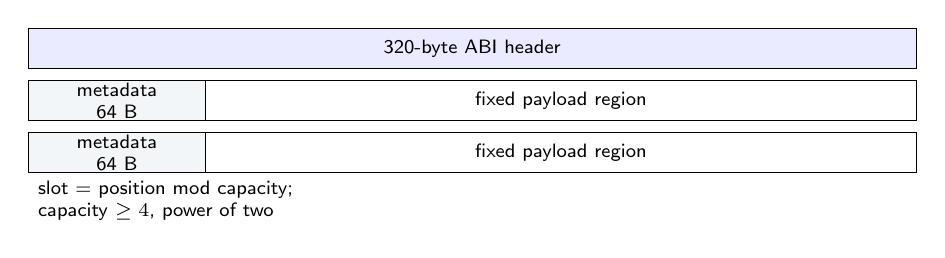
\begin{tikzpicture}[font=\scriptsize,x=.030\columnwidth,y=5.1mm]
\draw[fill=blue!8](0,0)rectangle(31,1)node[midway]{320-byte ABI header};
\draw[fill=light](0,-1.3)rectangle(6.2,-.3)node[midway,align=center]{metadata\\64 B};
\draw[fill=white](6.2,-1.3)rectangle(31,-.3)node[midway]{fixed payload region};
\draw[fill=light](0,-2.6)rectangle(6.2,-1.6)node[midway,align=center]{metadata\\64 B};
\draw[fill=white](6.2,-2.6)rectangle(31,-1.6)node[midway]{fixed payload region};
\node[align=left,anchor=west]at(0,-3.3){slot = position mod capacity;\\capacity $\geq4$, power of two};
\end{tikzpicture}
\caption{Shared segment layout. Serialization targets the selected slot's fixed backing region.}\label{fig:abi}
\end{figure}

The gateway's FlatBuffers builder uses a fixed, non-growing allocator over that
payload. Allocation either fits or the request is rejected before queue
reservation. Zero-copy is limited to the gateway--daemon handoff: no intermediate
serialized \code{Vec} is created, but parsing and other system copies remain.
FlatBuffers documents custom allocation in its Rust builder API
\cite{flatbuffersrust}. Fixed layout, bounds, and version validation remain
necessary; shared memory is not a trust boundary. The daemon bounds-checks the
slot-relative range, verifies the \code{FRTX} buffer with the generated C++
binding, checks required strings and request-ID agreement, and then borrows
views into the slot without materializing a request object.

\section{No-allocation daemon and SLA batcher}
The scheduler hot path owns no growing containers. It uses a fixed-capacity array
of slot pointers, a preallocated pool for eligible temporary memory, and a
\code{noexcept} handler. The native tests replace global allocation operators
and assert no allocation during one \code{poll\_once()} call. This is a narrow
implementation assertion, not a claim that metrics, drivers, logging, or every
production scoring component never allocates. Graph replay is separately
designed to avoid per-replay stream creation and host allocation after startup.

The continuous batcher drains ready slots to a maximum of 32 in the daemon
executable. It calls the handler when full or when the oldest element has waited
at least its configured 2 ms deadline. For oldest enqueue time $e_0$, monotonic
time $t$, capacity $B$, and staged count $n$, the trigger is
\[
(n=B)\lor(t-e_0\geq D),\qquad 0<n\leq B .
\]
This bounds scheduler waiting only if \code{poll\_once()} is called frequently.
It does not bound store work, GPU work, OS scheduling, or end-to-end response
latency. Full-batch and deadline-batch counters let experiments relate throughput
to the trigger that dispatched each batch.

\section{Lock-free ring correctness}
The ring is in the per-cell sequence-number family of bounded MPMC queues
\cite{lamport1977,michael1996}. A producer observes enqueue position $p$, claims
it by compare-and-exchange only when the slot sequence equals $p$, writes its
payload and metadata, then release-publishes $p+1$. A consumer claims $p$ after
acquire-observing $p+1$. Completion writes the response and release-publishes
$p+2$. The original producer owns that response until it copies it and stores
$p+C$, releasing the slot for the next ring generation, where $C$ is capacity.

\begin{figure}[t]\centering
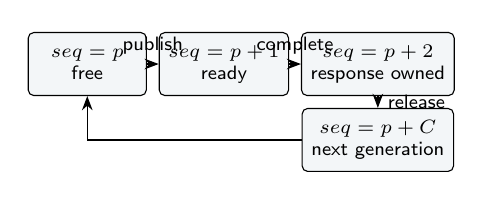
\begin{tikzpicture}[font=\scriptsize,node distance=1.5mm,
state/.style={draw,rounded corners=2pt,fill=light,align=center,minimum width=15mm,minimum height=8mm},
arr/.style={-{Stealth[length=1.8mm]},line width=.5pt}]
\node[state](a){$seq=p$\\free};\node[state,right=of a](b){$seq=p+1$\\ready};
\node[state,right=of b](c){$seq=p+2$\\response owned};
\node[state,below=of c](e){$seq=p+C$\\next generation};
\draw[arr](a)--node[above]{publish}(b);
\draw[arr](b)--node[above]{complete}(c);
\draw[arr](c)--node[right]{release}(e);
\draw[arr](e.west)-|(a.south);
\end{tikzpicture}
\caption{Per-slot state progression for absolute position $p$. A response cannot be overwritten before its producer releases it.}\label{fig:ring}
\end{figure}

The argument is deliberately narrow. Unique CAS ownership prevents duplicate
claims. Release/acquire synchronization exposes preceding writes to the acquirer.
The completed state prevents early response overwrite. Power-of-two capacity and
absolute positions distinguish generations in the intended range. Tests exercise
concurrent production, consumption, and wraparound, but are neither a formal
proof nor a cross-architecture memory-model proof. A crashed producer may leave
a hole; abandoned-slot recovery needs a separate protocol. Lock freedom here
does not mean the feature store, GPU driver, handler, or network cannot block.
\section{CUDA Graph and CUTLASS methodology}
CUDA Graphs can reduce repeated CPU launch overhead by capturing a stable
operation sequence and replaying an instantiated executable graph. This design
pre-captures batch sizes 1 through 32 with persistent nonblocking streams and
host/device buffers. The captured reference sequence is H2D copy, forward stub,
and D2H copy. CUDA defines graph capture and asynchronous execution semantics
that a benchmark must honor \cite{cudagraphs,cudaasync}.

This is a methodology hook, not evidence that the exported model uses graph
replay. A valid experiment compares identical shapes and buffers in direct and
replay modes after warmup, separately reports capture cost and uncaptured-shape
misses, and uses CUDA events for kernel/GPU-interval timing. Nsight Systems and
Compute establish launch behavior, occupancy, memory traffic, and stall reasons
\cite{nsight}.

CUTLASS is optional rather than silently substituted at runtime. The current
wrapper configures an SM80 TensorOp INT8-to-INT32 GEMM with 128$\times$128$\times$64
threadblock, 64$\times$64$\times$64 warp, and 16$\times$8$\times$32 instruction
shapes. CUTLASS supplies composable CUDA GEMM kernels \cite{cutlass}; its presence
does not establish model numerical equivalence, cuBLASLt comparison, or Tensor
Core throughput on a named device. FP8 candidates must measure score drift and
decision flips against FP32. FP8 formats and scaling trade-offs are described by
Micikevicius et al. \cite{fp8}. The current E4M3 code uses FP8
storage/conversion with FP32 accumulation and makes no Tensor Core throughput
claim.

\section{Load methodology: Poisson and HDR}
The load generator uses seeded exponential inter-arrival times: an open-loop
Poisson process with mean rate $\lambda$. Latency begins at the \emph{planned}
arrival, not worker admission, retaining saturation-induced client queueing.
Concurrency bounds in-flight sockets/goroutines without replacing the arrival
process. Entity mix, rate, duration or request count, and seed are run inputs.

HDR Histogram records every completion, including transport failures and non-2xx
responses, with status counts kept separately. Because observations start at
planned arrivals, the tester uses \code{RecordValue}, not synthetic coordinated-
omission correction. HDR Histogram is designed for wide ranges at controlled
precision \cite{hdr}. Report offered load, achieved throughput, error/fallback
rate, warmup, duration, and per-phase delay, not only a favorable percentile.
Orca provides context for iteration-level scheduling and selective batching in
latency-sensitive inference serving \cite{orca}. Triton's dynamic batching
documentation is a comparison point for batching policies, not a claim of
Triton equivalence \cite{tritonbatch}.

\begin{table*}[t]\centering\small
\caption{Minimum reproducibility record. A benchmark is incomplete if required fields are absent.}\label{tab:manifest}
\begin{tabularx}{\textwidth}{@{}p{.20\textwidth}Yp{.16\textwidth}Y@{}}\toprule
Category & Required fields & Category & Required fields \\\midrule
Identity & commit, UTC time, raw artifact paths & Hardware & CPU, GPU/count, network \\
Software & OS, driver, CUDA, compiler & Model & immutable hash, shape, backend \\
Load & duration, warmup, rate, seed, arrival, queue cap & Outcomes & percentiles, throughput, errors, fallbacks \\
Comparison & equal corpus/shapes, five repeats & Profiling & CUDA events, Nsight, cold/warm split \\\bottomrule
\end{tabularx}\end{table*}

\section{Results: checked-in evidence only}
% Generated by scripts/generate_research_figures.py; do not edit.
\newcommand{\ResultEvidenceStatus}{3 completed measured configuration(s) were generated from checked-in manifests; scope labels below are binding.}
\newcommand{\ResultEvidenceFigure}{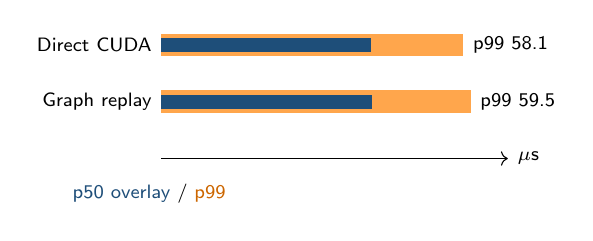
\begin{tikzpicture}[font=\scriptsize]\begin{scope}[x=0.06603cm,y=.72cm,xshift=1.25cm]\draw[->] (0,0)--(66.640,0) node[right]{$\mu$s};\node[anchor=east] at (0,2) {Direct CUDA};\fill[orange!70] (0,1.8) rectangle (58.1,2.2);\fill[accent] (0,1.88) rectangle (40.4,2.12);\node[anchor=west] at (58.1,2) {p99 58.1};\node[anchor=east] at (0,1) {Graph replay};\fill[orange!70] (0,0.8) rectangle (59.5,1.2);\fill[accent] (0,0.88) rectangle (40.5,1.12);\node[anchor=west] at (59.5,1) {p99 59.5};\end{scope}\node[anchor=west] at (0,-.45) {\textcolor{accent}{p50 overlay} / \textcolor{orange!80!black}{p99}};\end{tikzpicture}}
\begin{table*}[t]
\centering
\caption{Measured summaries generated from checked-in JSON manifests.}
\label{tab:generated-results}
\scriptsize
\begin{tabularx}{\textwidth}{@{}lllXrrrr@{}}
\toprule
Artifact & Commit & Backend & Scope & p50 ($\mu$s) & p99 ($\mu$s) & Rate/s & Errors \\
\midrule
CUDA direct runs & 2627824c & Direct CUDA & CPU wall time per warmed direct batch-32 H2D/forward/D2... & 40.4 & 58.1 & -- & 0.00\% \\
CUDA graph runs & 2627824c & Graph replay & CPU wall time per warmed batch-32 replay, including cud... & 40.5 & 59.5 & -- & 0.00\% \\
Linux HTTP/IPC run & d71b52fd & HTTP + IPC & planned open-loop client arrival through authenticated ... & 2325 & 3421 & 1505.70 & 0.00\% \\
\bottomrule
\end{tabularx}
\end{table*}
\newcommand{\NsightEvidenceStatus}{Nsight Systems observed positive host/GPU overlap in 500 of 500 bounded probes; median overlap was 362 ns.}
\newcommand{\NsightEvidenceFigure}{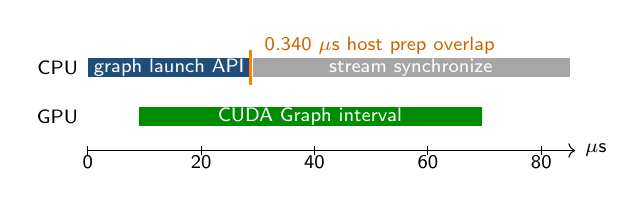
\begin{tikzpicture}[font=\scriptsize,x=.072cm,y=.62cm]
\node[anchor=east] at (0,2) {CPU}; \node[anchor=east] at (0,1) {GPU};
\fill[accent] (0,1.8) rectangle (28.739,2.2);
\node[white] at (14.37,2) {graph launch API};
\fill[green!55!black] (8.987,.8) rectangle (69.467,1.2);
\node[white] at (39.2,1) {CUDA Graph interval};
\draw[orange,line width=1.2pt] (28.739,1.65)--(28.739,2.35);
\node[anchor=west,orange!80!black] at (29.5,2.45) {0.340 $\mu$s host prep overlap};
\fill[gray!70] (29.079,1.8) rectangle (84.988,2.2);
\node[white] at (57.0,2) {stream synchronize};
\draw[->] (0,.3)--(86,.3) node[right] {$\mu$s};
\foreach \x in {0,20,40,60,80}{\draw (\x,.2)--(\x,.4) node[below] {\x};}
\end{tikzpicture}}
% CSV artifacts detected: cuda_component_runs_2627824.csv, d71b52f-run-30587168363-distribution.csv, nsys_timeline_2627824.csv

\ResultEvidenceStatus

\begin{figure}[t]\centering\ResultEvidenceFigure
\caption{Comparable local CUDA component percentiles generated from checked-in
manifests. The generated table also reports the separately scoped Linux API
run; targets are never interpolated into either view.}\label{fig:results}
\end{figure}

At commit \code{2627824c}, five independently launched component runs each used
100 warmups and 2,000 observations on an RTX 3050. Median run summaries were
p50/p99 40.4/58.1~$\mu$s for direct execution and 40.5/59.5~$\mu$s for graph
replay. Thus CUDA Graph replay did not improve p50 or p99 for this deliberately
small stub. Compute Sanitizer reported zero errors, and the single CUTLASS
INT8--INT32 GEMM matched its CPU reference exactly; neither establishes model
accuracy or sustained Tensor Core throughput.

At commit \code{d71b52fd}, a GitHub-hosted four-vCPU AMD EPYC runner drove one
seeded open-loop Poisson run through Rust HTTP parsing, direct FlatBuffer
serialization, System V IPC, C++ FRTX verification/decoding, the scheduler, and
the CPU reference handler. All 15,000 requests returned HTTP 200. Achieved
throughput was 1,505.70/s; p50, p90, p99, p99.9, and maximum planned-arrival-to-
completion latency were 2.325, 3.145, 3.421, 3.939, and 4.943~ms. This is an
observational integration run, not a capacity limit or repeated comparison.

\begin{figure}[t]\centering
\NsightEvidenceFigure
\caption{Measured Nsight Systems sample on the RTX 3050. The host prepared
bounded response metadata after \code{cudaGraphLaunch} returned and before
synchronization; the 0.340~$\mu$s interval lies inside the device graph interval.
This is real but too small to imply an end-to-end speedup.}\label{fig:nsight}
\end{figure}
\NsightEvidenceStatus{} Nsight Systems also found asynchronous H2D API return
before device-copy completion in 2,093 of 2,100 joined calls. Nsight Compute
hardware counters were unavailable under \code{ERR\_NVGPUCTRPERM}; occupancy,
Tensor Core utilization, cache traffic, and stall metrics are therefore not
claimed.

The Linux workflow also retained 4,988 daemon-only \code{perf} samples, folded
stacks, and a rendered flame graph. Sampled time is dominated by the polling
loop, monotonic clock reads, and scheduler yielding; no allocation symbol appears
in the folded sample. This supports---but cannot prove---the hot-path allocation
claim, because sampling can miss short calls and excludes the gateway and client.
The allocation-counting unit test is the direct regression guard. The SVG,
folded stacks, profiler diagnostics, and provenance are checked in under
\code{docs/profiling/results/}.

Performance promotion is a gated experiment: at least five repeated runs should
show numerical tolerance, no API p99 regression at equal offered load, bounded
deadline-miss/fallback rate, and tested capability fallback. MLPerf Inference is
a useful reference for controlled scenarios, accuracy constraints, and reporting
discipline \cite{mlperfinference}; this project does not claim MLPerf compliance.
\section{Threats, limitations, and reproducibility}
\textbf{Model validity.} Deterministic/synthetic lifecycle material does not
establish production fraud quality, fairness, calibration under drift, or
economic cost. TabTransformer motivates contextual tabular modeling but does not
validate this feature set or model \cite{tabtransformer}.

\textbf{Systems validity.} The local worker is a deterministic scorer, not the
exported transformer. The graph path captures a forward stub. System V IPC is
Linux-specific, and CPU/GPU timing is not API timing. Warm co-located results
would not generalize to remote clients, cache misses, contention, driver changes,
or failure recovery.

\textbf{Concurrency validity.} Lock freedom applies to the bounded ring's
progress condition, not to the whole deployment. The batch handler, feature
store, GPU driver, memory allocator outside the guarded scheduler, and network
may block. Tests are valuable regressions, but no formal linearizability proof
or cross-process model checking is provided.

\textbf{Security and operations.} Mode-0600 constrains segment access but does
not authenticate a compromised local process. Production still needs host
hardening, secret rotation, signed models, access control, safe telemetry, and
reviewable fallback policy. Fail-closed behavior trades availability for
integrity when trustworthy features are absent.

To reproduce an eventual claim: (1) build a named commit and record hardware,
software, capability selection, and model hash; (2) warm keys and graph variants,
while retaining cold runs separately; (3) drive seeded Poisson load and collect
HDR histograms, quantile CSVs, status counts, CUDA events, and Nsight exports;
(4) place completed JSON/CSV artifacts under \code{docs/profiling/results/};
and (5) run \code{python scripts/generate\_research\_figures.py} before compiling
this paper. Compare baseline/candidate at equal offered load and corpus, retain
failed runs, and impair a worker/store. The checked-in artifacts now satisfy
this protocol for the two narrow scopes reported above. Inputs still needed
before a production conclusion are a real model bundle and corpus, repeated
paired API baselines, cold-start and failure runs, numerical decision-drift
analysis, and permitted Nsight Compute counters.

\section{Conclusion}
This design makes ownership explicit at the shared-memory boundary, keeps the
daemon scheduler bounded and allocation-aware, uses an SLA batch trigger, and
treats CUDA Graph/CUTLASS integrations as experiments rather than performance
slogans. Its most useful current component result is negative: graph replay did
not improve the p50 or p99 of the tiny launch-dominated stub. The CPU-only Linux
run demonstrates the complete authenticated HTTP-to-shared-memory protocol at
the stated load, while deliberately stopping short of a production-model or
capacity claim. Keeping targets separate from measured scope leaves a clear
route to credible evaluation.

\section{Evaluation matrix for future runs}
The purpose of an evaluation matrix is to prevent a system change from being
credited for a difference caused by another changed variable. Every row below
is a required comparison, not an existing measurement. The baseline and
candidate must use the same request corpus, model bundle, feature shape, offered
load, warmup rule, and error policy. The output is written to the machine-
readable manifest only after raw artifacts are preserved.

\begin{table}[t]\centering\scriptsize
\caption{Required comparisons before a latency or throughput conclusion.}\label{tab:matrix}
\begin{tabularx}{\columnwidth}{@{}lY Y@{}}\toprule
Experiment & Controls and candidate & Required observations \\\midrule
CPU reference & fixed corpus, shape, load; FP32 handler & API percentiles, errors, fallback, CPU saturation \\
CUDA direct & same warmed buffers; direct H2D/forward/D2H & kernel and GPU interval, drift, capability \\
Graph replay & same CUDA inputs; captured batch 1--32 & replay, capture cost, misses, API p99 \\
CUTLASS GEMM & same matrices/tolerance; optional INT8 & correctness, throughput, occupancy, traffic \\
Batching & same offered rate; batcher versus one & queue delay, trigger counts, p99, throughput \\
Failure path & same workload; worker/store impairment & misses, fallbacks, recovery, provenance \\\bottomrule
\end{tabularx}\end{table}

An API conclusion must remain distinct from a component conclusion. CUDA events
can demonstrate a kernel or GPU interval only; they cannot measure request
parsing, feature retrieval, socket queueing, scheduler delay, response encoding,
or the client network path. Conversely, an API percentile without phase
breakdown cannot establish why it changed. The protocol therefore records both
types of evidence and labels their scope at report time.

\begin{figure}[b]\centering
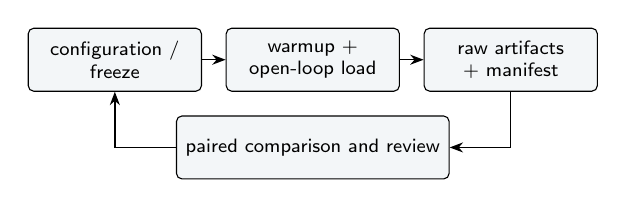
\begin{tikzpicture}[font=\scriptsize,node distance=3mm,
n/.style={draw,rounded corners=2pt,fill=light,minimum width=22mm,minimum height=8mm,align=center},
a/.style={-{Stealth[length=1.7mm]},line width=.5pt}]
\node[n](one){configuration /\\freeze};
\node[n,right=of one](two){warmup +\\open-loop load};
\node[n,right=of two](three){raw artifacts\\+ manifest};
\node[n,below=of two](four){paired comparison and review};
\draw[a](one)--(two);\draw[a](two)--(three);\draw[a](three.south)|-(four.east);\draw[a](four.west)-|(one.south);
\end{tikzpicture}
\caption{Evidence loop for each optimization. A result is reviewable only after configuration, raw artifacts, and paired comparison agree.}
\end{figure}

\clearpage
\section{Numerical and decision-integrity protocol}
Latency optimization is not useful if it changes decisions silently. The FP32
reference serves as a component-level oracle for finite inputs. Any FP16, FP8,
or INT8 candidate must declare its calibration/tolerance policy before the run,
then report absolute and relative score error, changed decision count, changed
explanation count where applicable, and all non-finite outputs. A capability
failure must recompute or report the documented fallback; it must not be labeled
as a successful accelerated result merely because a device advertises support.

\begin{table}[t]\centering\scriptsize
\caption{Decision-integrity evidence to retain beside timing artifacts.}\label{tab:numeric}
\begin{tabularx}{\columnwidth}{@{}lY Y@{}}\toprule
Item & Evidence & Rejection condition \\\midrule
Reference inputs & immutable corpus ID, seed, fixed feature shape & corpus differs across compared paths \\
Calibration & bundle hash, thresholds, precision/scales, declared tolerances & undeclared recalibration after observing output \\
Scores & max absolute/relative error, distribution summary, non-finite count & tolerance breach or unexplained non-finite \\
Decisions & allow/review/decline confusion matrix and changed request IDs & unreviewed decision flip \\
Fallback & device capability, reason, backend reported to caller & fallback counted as accelerated primary result \\
Repeatability & five paired runs and artifact hashes & a favorable single run is presented as conclusive \\\bottomrule
\end{tabularx}\end{table}

This policy is especially important for FP8. The project may use E4M3 storage
with FP32 accumulation on capable hardware, but that implementation fact does
not certify accuracy or Tensor Core performance. The FP8 literature establishes
formats and scaling techniques, not this deployment's calibration \cite{fp8}.
The same separation applies to tabular-model literature: TabTransformer is
motivation for architecture choices, not evidence of fraud quality here
\cite{tabtransformer}.

\clearpage
\section{Failure and tail-latency runbook}
Tail behavior must be measured under steady load and under controlled loss. The
following injections are bounded and reversible in a test environment. They
should never be executed against a live authorization service without an
approved safety plan. The expected behavior is an observable deadline/fallback
transition, not a silent extension of the caller deadline.

\begin{table}[t]\centering\scriptsize
\caption{Controlled impairment plan for the warm decision path.}\label{tab:failures}
\begin{tabularx}{\columnwidth}{@{}lY Y@{}}\toprule
Impairment & Injection and expected behavior & Record \\\midrule
Worker removal & router opens circuit; reroute or fallback & route, reason, remaining deadline \\
Feature-store delay & child deadline; fail closed without features & phase delay, status, decision \\
Ring saturation & bounded reject/queue deadline; no corrupt slot & depth, sequence, error count \\
CUDA capability loss & explicit CPU/fallback; no false acceleration & capability, backend, score drift \\
Graph miss & direct path or explicit unavailable state & graph status, batch size, timing scope \\
Client overload & planned-arrival latency exposes queueing & offered/achieved rate, HDR percentile \\\bottomrule
\end{tabularx}\end{table}

Tail aggregation must report each population separately: warm primary success,
cold or uncaptured startup, explicit fallback, feature failure, timeout, and
transport error. Combining them can conceal a failure mode or make a healthy
subpopulation look worse than its contract. The design follows the tail-at-scale
principle by treating the rare slow path as a first-class result rather than
discarding it \cite{dean2013}.

\clearpage
\appendix
\section{Experiment reporting sheet}
This appendix is intentionally a printable reporting aid rather than an
evaluation. It makes the evidence required for a future claim visible before a
benchmark is run. Copy it into each experiment record together with raw files.

\begin{table*}[h]\centering\small
\caption{Run identity and environment sheet. Empty cells are missing evidence, not defaults.}
\begin{tabularx}{\textwidth}{@{}p{.20\textwidth}Yp{.16\textwidth}Y@{}}\toprule
Field & Value & Field & Value \\\midrule
Commit & \rule{.28\textwidth}{.35pt} & UTC started & \rule{.22\textwidth}{.35pt}\\[7pt]
Model bundle hash & \rule{.28\textwidth}{.35pt} & Backend/path & \rule{.22\textwidth}{.35pt}\\[7pt]
CPU / RAM & \rule{.28\textwidth}{.35pt} & GPU / count & \rule{.22\textwidth}{.35pt}\\[7pt]
OS / kernel & \rule{.28\textwidth}{.35pt} & Driver / CUDA & \rule{.22\textwidth}{.35pt}\\[7pt]
Network & \rule{.28\textwidth}{.35pt} & Compiler & \rule{.22\textwidth}{.35pt}\\[7pt]
\bottomrule\end{tabularx}\end{table*}

\begin{table*}[h]\centering\small
\caption{Load and outcome sheet. Keep cold and warm populations separate.}
\begin{tabularx}{\textwidth}{@{}p{.20\textwidth}Yp{.16\textwidth}Y@{}}\toprule
Field & Value & Field & Value \\\midrule
Arrival distribution / seed & \rule{.28\textwidth}{.35pt} & Offered rate & \rule{.22\textwidth}{.35pt}\\[7pt]
Duration / warmup & \rule{.28\textwidth}{.35pt} & Queue cap & \rule{.22\textwidth}{.35pt}\\[7pt]
Corpus / entity mix & \rule{.28\textwidth}{.35pt} & Concurrency cap & \rule{.22\textwidth}{.35pt}\\[7pt]
p50 / p95 / p99 / p99.9 & \rule{.28\textwidth}{.35pt} & Maximum & \rule{.22\textwidth}{.35pt}\\[7pt]
Throughput / errors / fallbacks & \rule{.28\textwidth}{.35pt} & Raw paths & \rule{.22\textwidth}{.35pt}\\[7pt]
\bottomrule\end{tabularx}\end{table*}

\section{Measurement decision checklist}
\begin{enumerate}
\item Is the profiling manifest complete and checked in with raw HDR, CSV, and
profiler artifacts?
\item Does the comparison use the same model hash, request corpus, shape,
warmup rule, offered load, and latency scope?
\item Are failed runs, error rate, fallback rate, maximum, and cold runs
reported separately rather than discarded?
\item Is an optimization claim limited to hardware and software actually named
in the manifest?
\item Did numerical tolerances and decision flips pass before performance
promotion?
\item Is the result reproducible at least five times and has the fallback path
been exercised on unsupported capability or injected impairment?
\end{enumerate}

\section{Artifact schema}
A completed JSON manifest should use the repository schema version, record
commit and timestamp, provide CPU/GPU/network and OS/CUDA/driver/compiler
details, identify the immutable model bundle and fixed shape, and describe
duration, warmup, request rate, Poisson arrival, and queue delay. Its results
must include latency percentiles, maximum, throughput, error rate, and fallback
rate. The generator ignores null results intentionally. CSV quantiles and raw
HDR/NSight files should reside beside the manifest or be referenced by stable
repository paths.

\clearpage
\begin{thebibliography}{99}\small
\bibitem{dean2013} J. Dean and L. A. Barroso. The Tail at Scale. \textit{CACM}, 56(2), 2013. \url{https://doi.org/10.1145/2408776.2408794}
\bibitem{cudagraphs} NVIDIA. CUDA Graphs, \textit{CUDA C++ Programming Guide}. \url{https://docs.nvidia.com/cuda/cuda-c-programming-guide/index.html\#cuda-graphs}
\bibitem{cudaasync} NVIDIA. Asynchronous Concurrent Execution, \textit{CUDA C++ Programming Guide}. \url{https://docs.nvidia.com/cuda/cuda-c-programming-guide/index.html\#asynchronous-concurrent-execution}
\bibitem{cutlass} NVIDIA. \textit{CUTLASS}. \url{https://github.com/NVIDIA/cutlass}
\bibitem{flatbuffersrust} Google. Rust usage, \textit{FlatBuffers documentation}. \url{https://flatbuffers.dev/languages/rust/}
\bibitem{linuxshmget} Linux man-pages. \textit{shmget(2)}. \url{https://man7.org/linux/man-pages/man2/shmget.2.html}
\bibitem{linuxshmat} Linux man-pages. \textit{shmat(2)}. \url{https://man7.org/linux/man-pages/man2/shmat.2.html}
\bibitem{hdr} G. Tene. \textit{HdrHistogram}. \url{https://hdrhistogram.github.io/HdrHistogram/}
\bibitem{orca} G.-I. Yu et al. Orca: A Distributed Serving System for Transformer-Based Generative Models. \textit{OSDI}, 2022. \url{https://www.usenix.org/conference/osdi22/presentation/yu}
\bibitem{mlperfinference} V. J. Reddi et al. MLPerf Inference Benchmark. arXiv:1911.02549, 2019. \url{https://arxiv.org/abs/1911.02549}
\bibitem{lamport1977} L. Lamport. Proving the Correctness of Multiprocess Programs. \textit{IEEE TSE}, 1977. \url{https://doi.org/10.1109/TSE.1977.229904}
\bibitem{michael1996} M. M. Michael and M. L. Scott. Simple, Fast, and Practical Non-Blocking and Blocking Concurrent Queue Algorithms. PODC, 1996. \url{https://doi.org/10.1145/248052.248106}
\bibitem{tabtransformer} X. Huang et al. TabTransformer. arXiv:2012.06678, 2020. \url{https://arxiv.org/abs/2012.06678}
\bibitem{fp8} P. Micikevicius et al. FP8 Formats for Deep Learning. arXiv:2209.05433, 2022. \url{https://arxiv.org/abs/2209.05433}
\bibitem{tritonbatch} NVIDIA. Dynamic Batching, \textit{Triton Inference Server User Guide}. \url{https://docs.nvidia.com/deeplearning/triton-inference-server/user-guide/docs/user_guide/batcher.html}
\bibitem{nsight} NVIDIA. \textit{Nsight Systems and Nsight Compute Documentation}. \url{https://docs.nvidia.com/nsight-systems/} \url{https://docs.nvidia.com/nsight-compute/}
\end{thebibliography}
\end{document}
